% !TEX encoding = UTF-8
% !TEX TS-program = pdflatex
% !TEX root = ../tesi.tex

%**************************************************************
\chapter{Analisi dei requisiti}
\label{cap:analisi_dei_requisiti}
%**************************************************************
In questo capitolo verranno esposti i casi d'uso e i requisiti del modulo \gls{ITF} che erano oggetto del lavoro di stage.\\
Si procede con la descrizione dello stato del sistema, gli attori che vi partecipano, le pre-condizioni, le post-condizioni e gli scenari.\\
I casi d'uso principali sono associati ad un diagramma \gls{uml} 2.0 che riporta lo stesso codice identificativo e titolo del caso d'uso al quale si riferisce.

%**************************************************************
\section{Dominio}
\subsection{Caratteristiche degli attori}
L'interazione con il modulo \gls{ITF} coinvolge essenzialmente tre tipologie diverse di attori:
\begin{itemize}
	\item L'identity wallet;
	\item Un ente certificatore;
	\item Un service provider.
\end{itemize}

\subsubsection{Identity Wallet}
Questa componente del sistema ha il compito di generare, mantenere e presentare l'identità digitale dell'utente. A sua volta, l'\textit{Identity Wallet} interagisce con il sistema \gls{ITF} nel momento in cui un utente esegue una richiesta di accesso verso un \textit{service provider} il quale richiede l'autenticazione e la conferma delle credenziali insieme alla verifica di attributi specifici necessari per erogare i suoi servizi.\\
Il sistema \gls{monokee}, una volta che l'utente richiede l'accesso ad un \textit{service provider}, reindirizza la richiesta di accesso all'\gls{ITF}.
\subsubsection{Ente Certificatore (Trusted Third Party)}
La seconda tipologia di attori che interagiscono con il sistema da realizzare sono i \textit{Trusted Third Party}.\\
Questi, chiamati enti certificatori, hanno il compito di certificare le informazioni che sono presenti all'interno dell'\gls{ITF} in modo che, ogni qual volta che vengono richieste informazioni per poter accedere ad un \textit{service provider}, le informazioni che il sistema fornisce per l'autenticazione e/o l'erogazione di servizi, siano verificate da un ente esterno che garantisce la loro veridicità.
\subsubsection{Service Provider}
La terza e ultima tipologia di attori che partecipano al sistema sono i \textit{service provider}.
Questi interagiscono con l'\gls{ITF} durante la fase di verifica delle informazioni. Questi devono autenticare gli utenti tramite le loro credenziali e autorizzare l'erogazione di servizi dopo la verifica degli attributi
%**************************************************************
\subsection{Overview del sistema}
Una rappresentazione delle funzionalità che deve implementare il modulo \gls{ITF} può essere ripresa in figura \ref{fig:moduloITF}.\\\\
Il prodotto finale prevede l'interazione delle tre tipologie di attori allo scopo di garantire:
\begin{itemize}
	\item L'accesso sicuro al \textit{service provider} desiderato;
	\item L'erogazione dei servizi offerti dal \textit{service provider} in modo controllato.
\end{itemize}
Questo viene garantito dall'\gls{ITF} e dalla tecnologia \textit{Blockchain} che ne è alla base.\\
Di seguito viene descritto il flusso di chiamate che intercorrono affinchè un utente possa accedere ad uno o più servizi di sua scelta.\\\\
Quando un utente richiede dei servizi, da parte di un \textit{service provider}, il sistema viene interrogato e inizia lo scambio di informazioni che coinvolge l'\textit{identity wallet}, gli enti certifictori ed il \textit{service provider}.\\
Ogni qual volta un utente richiede l'accesso a dei servizi di un determinato \textit{service provider}, \gls{monokee} reindirizza la richiesta d'accesso all'\textit{identity wallet} che, a sua volta, invia la richiesta di accesso all'\gls{ITF} passandogli un identificativo dell'utente che ha fatto la richiesta di accesso insieme alle informazioni che il \textit{service provider} necessita per poter permettere l'erogazione dei suoi servizi.\\
Nell'\gls{ITF} viene eseguita una ricerca nella rete \textit{Blockchain} sottostante in modo da verificare se le informazioni richieste dal \textit{service provider} siano efffettivamente associate all'utente. Se il riscontro è positivo, il \textit{service provider} permette l'accesso all'utente altrimenti gli viene negato.\\\\
La seconda tipologia di attori che partecipano al sistema, gli enti certificatori, entrano in gioco durante la fase di registrazione di un nuovo utente o quando un amministratore di dominio associa degli attributi alle identità digitali dei suoi utenti.
Gli enti certificatori hanno il compito di verificare e certificare che, le asserzioni o gli attributi, di una particolare identità, siano conformi alle informazioni associate a quell'utente.\\
Questo ruolo è di fondamentale importanza all'interno del sistema che si sta sviluppando in quanto, essendo l'\gls{ITF} basata su una \textit{Blockchain}, tutte le informazioni che popolano la rete sono immutabili e, quindi, prima di essere definitivamente inserite in un blocco, devono essere verificate e approvate, dagli enti certificatori, tramite gli algoritmi di consenso.\\\\
La terza tipologia di attori, i \textit{service providers}, interagiscono con il sistema durante la verifica delle informazioni dell'identità dell'utente.\\
Questi, dopo che l'\textit{identity wallet} gli ha passato i record contenenti la chiave pubblica e il riferimento alla locazione del record cifrato nell'\gls{ITF}, iniziano il  controllo delle informazioni.\\
Il controllo viene fatto andando prima a calcolare l'\textit{hash crittografico} della chiave pubblica pervenuta dall'\textit{identity wallet} e poi andando a confrontare il risultato ottenuto con quello presente nell'\gls{ITF} recuperato grazie al riferimento alla sua locazione nella rete Blockchain.
In questa fase, il \textit{service provider} verifica i record contenente l'identità e qualsiasi altra credenziale per autenticare l'utente e verifica anche gli attributi necessari per autorizzare l'utente ad utilizzare i suoi servizi.
\section{Casi d'uso}
\subsection{Classificazione dei casi d'uso}
Ogni caso d'uso è classificato secondo la seguente convienzione:\\\\
\centerline{UC[codicePadre]\_[codiceFiglio]}\\\\
In cui i due codici rappresentano:
\begin{itemize}
	\item \textbf{codicePadre} - identifica univocamente il caso d'uso;
	\item \textbf{codiceFiglio} - identifica univocamente i sotto casi d'uso apparteneti ad un determinato "codicePadre".
\end{itemize}

\subsection{Descrizione dei casi d'uso}
Ogni caso d'uso viene descritto dalla seguente struttura:
\begin{itemize}
	\item \textbf{Descrizione} - Breve descrizione del caso d'uso che si sta modellando;
	\item \textbf{Attori Principali} - Indica l'attore principale del caso d'uso. In tutto il contesto dell'applicazione, gli attori saranno classificati come:
	\begin{itemize}
		\item Identity Wallet;
		\item Trusted Third Party (ente certificatore);
		\item Service Provider.
	\end{itemize}
	\item \textbf{Attori Secondari} - Indica l'attore che aiuta l'attore principale a realizzare quanto descritto dal caso d'uso;
	\item \textbf{Pre-Condizioni} - Specifica la condizione del sistema prima del verificarsi degli eventi descritti dal caso d'uso;
	\item \textbf{Post-Condizioni} - Specifica le condizioni del sistema dopo il verificarsi degli eventi descritti dal caso d'uso;
	\item \textbf{Scenario Principale} - Rappresenta il flusso principale degli eventi ovvero il caso in cui tutto funzioni come deve;
	\item \textbf{Estensioni} - Rappresenta il flusso secondario degli eventi nel caso in cui si verifichino degli errori nel flusso principale.
\end{itemize}

\subsection{Caso d'uso UC1: Registrazione}
\begin{figure}[h]
	\centering
	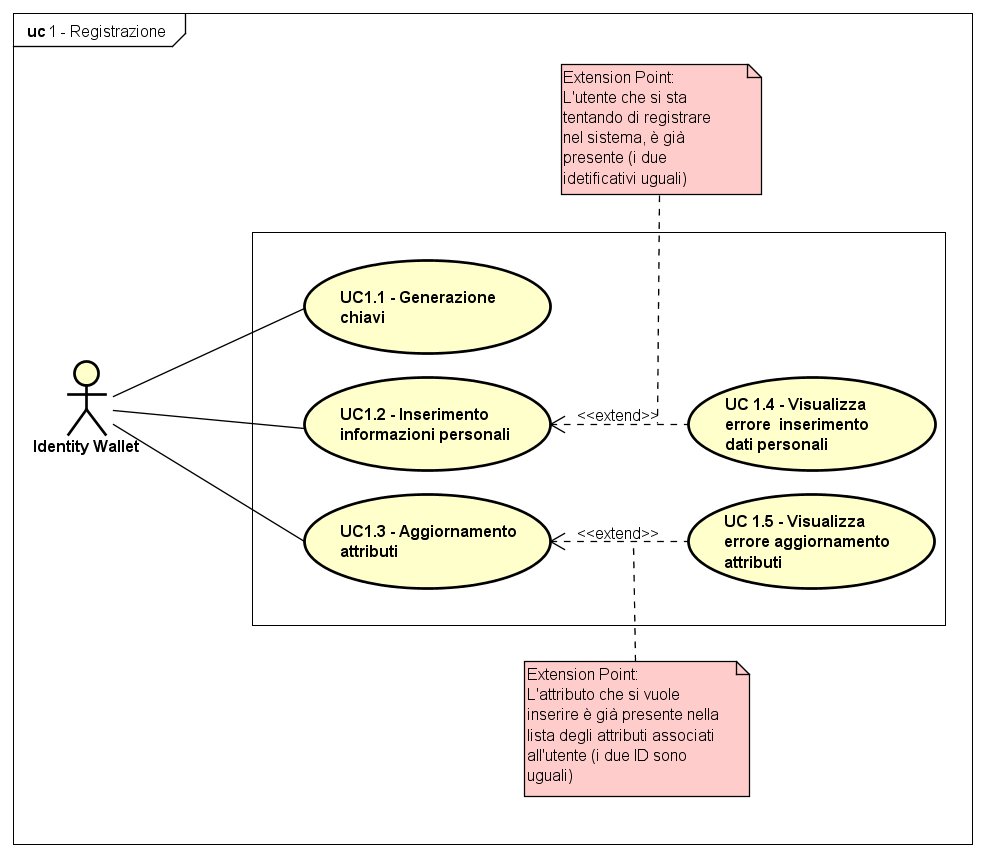
\includegraphics[scale=0.50]{immagini/usecase/UC1_Registrazione}
	\caption{Caso d'uso UC1: Registrazione}
\end{figure}
\begin{itemize}
	\item \textbf{Descrizione} - L'Identity Wallet genera la chiave pubblica, quella privata ed inserisce le informazioni personali dell'utente. In alternativa può aggiornare gli attributi esistenti aggiungendone di nuovi;
	\item \textbf{Attori Principali} - Identity Wallet;
	\item \textbf{Attori Secondari} -
	\item \textbf{Pre-Condizioni} - L'Identity Wallet non possiede un identità digitale per l'utente;
	\item \textbf{Post-Condizioni} - L'Identity Wallet ha creato un identità per l'utente ed è in attesa che questa venga certificata;
	\item \textbf{Scenario Principale} - 
	\begin{enumerate}
		\item Generazione delle chiavi (UC 1.1);
		\item Inserimento delle informazioni personali (UC 1.2);
		\item Aggiornamento degli attributi già presenti nell'\gls{ITF} (UC 1.3);
	\end{enumerate}
	\item \textbf{Estensioni} -
	\begin{enumerate}
		\item All'Identity Wallet viene segnalato un errore di registrazione del nuovo utente (UC 1.4);
		\item All'Identity Wallet viene segnalato un errore sull'aggiornamento degli attributi (UC 1.5).
	\end{enumerate}
\end{itemize}
\subsection{Caso d'uso UC1.1: Generazione Chiavi}
\begin{figure}[h]
	\centering
	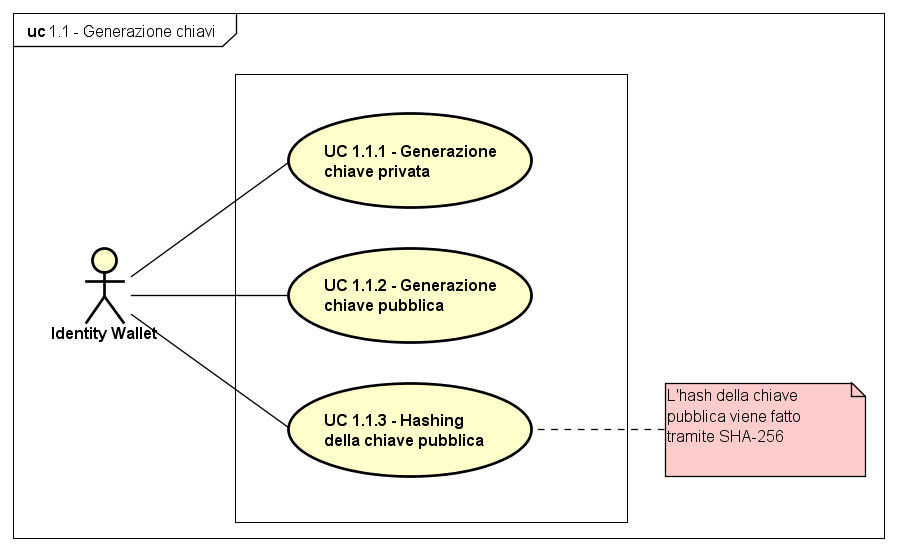
\includegraphics[scale=0.50]{immagini/usecase/UC11_GenerazioneChiavi}
	\caption{Caso d'uso UC1.1: Generazione chiavi}
\end{figure}
\begin{itemize}
	\item \textbf{Descrizione} - L'Identity Wallet genera la chiave privata e quella pubblica. Quest'ultima viene crittografata tramite \textit{hash} e rappresenta l'identità digitale dell'utente;
	\item \textbf{Attori Principali} - Identity Wallet;
	\item \textbf{Attori Secondari} -
	\item \textbf{Pre-Condizioni} - L'Identity Wallet non possiede una coppia di chiavi pubblica-privata;
	\item \textbf{Post-Condizioni} - L'Identity Wallet è in possesso di una coppia di chiavi (pubblica e privata) e del \textit{hash} di quella pubblica;
	\item \textbf{Scenario Principale} -
	\begin{enumerate}
		\item Generazione della chiave privata (UC 1.1.1);
		\item Generazione della chiave pubblica (UC 1.1.2);
		\item Generazione del \textit{hash} della chiave pubblica (UC 1.1.3).
	\end{enumerate}
	\item \textbf{Estensioni} -
\end{itemize}
\subsection{Caso d'uso UC1.2: Inserimento informazioni personali}
\begin{figure}[h]
	\centering
	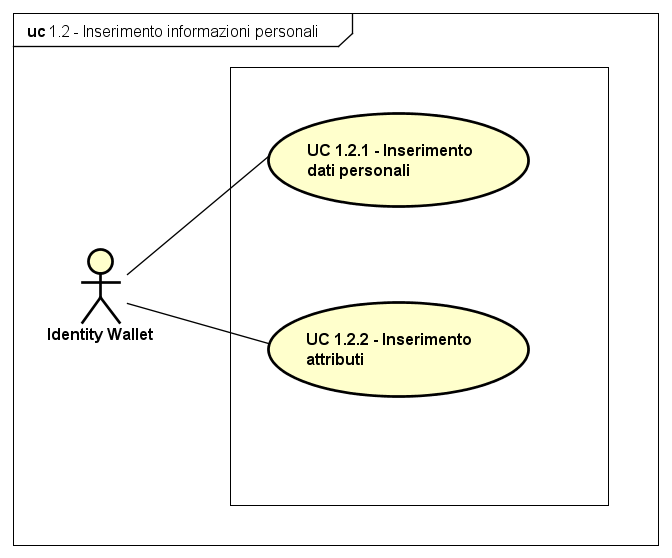
\includegraphics[scale=0.50]{immagini/usecase/UC12_InserimentoInformazioniPersonalii}
	\caption{Caso d'uso UC1.2: Inserimento informazioni personali}
\end{figure}
\begin{itemize}
	\item \textbf{Descrizione} - L'Identity Wallet crea l'identità digitale dell'utente come un insieme di dati personali e attributi a lui associati;
	\item \textbf{Attori Principali} - Identity Wallet;
	\item \textbf{Attori Secondari} -
	\item \textbf{Pre-Condizioni} - L'Identity Wallet non possiede le informazioni personali dell'utente ed i suoi attributi;
	\item \textbf{Post-Condizioni} - L'Identity Wallet possiede tutte le informazioni personali dell'utente ed i suoi attributi;
	\item \textbf{Scenario Principale} -
	\begin{enumerate}
		\item Inserimento dei dati personali utente (UC 1.2.1);
		\item Inserimento dei degli attributi utente (UC 1.2.2);
	\end{enumerate}
	\item \textbf{Estensioni} -
\end{itemize}
\subsection{Caso d'uso UC1.2.1: Inserimento dati personali utente}
\begin{figure}[h]
	\centering
	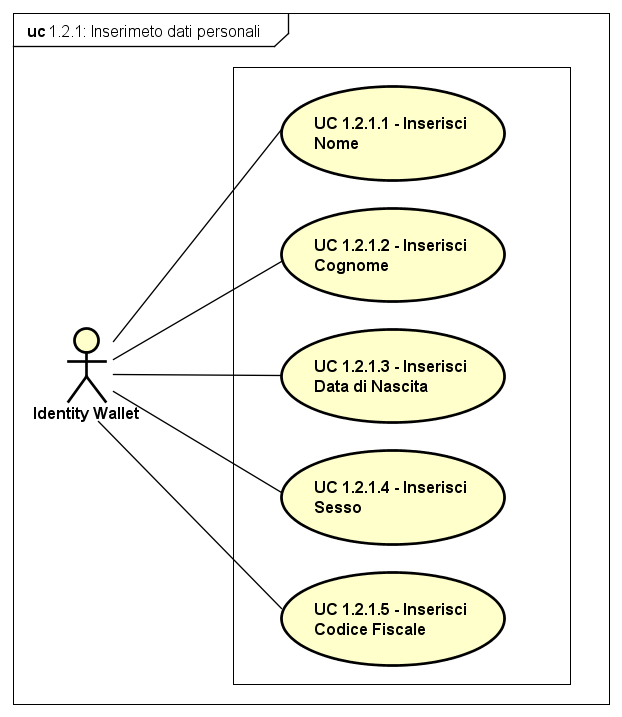
\includegraphics[scale=0.50]{immagini/usecase/UC121_InserimentoDatiPersonali}
	\caption{Caso d'uso UC1.2.1: Insierimento dati personali utente}
\end{figure}
\begin{itemize}
	\item \textbf{Descrizione} - L'Identity Wallet compila i campi dedicati alle informazioni personali dell'identità utente che vuole registrare all'ITF;
	\item \textbf{Attori Principali} - Identity Wallet;
	\item \textbf{Attori Secondari} -
	\item \textbf{Pre-Condizioni} - L'Identity Wallet non ha inserito le informazioni personali dell'identità utente che vuole registrare nell'\gls{ITF};
	\item \textbf{Post-Condizioni} - L'Identity Wallet ha inserito tutte le informazioni personali dell'identità utente che vuole registrare nell'\gls{ITF};
	\item \textbf{Scenario Principale} -
	\begin{enumerate}
		\item Inserimento del nome dell'utente (UC 1.2.1.1);
		\item Inserimento del cognome dell'utente (UC 1.2.1.2);
		\item Inserimento della data di nascita (UC 1.2.1.3);
		\item Inserimento del sesso dell'utente (UC 1.2.1.4);
		\item Inserimento del codice fiscale (UC 1.2.1.5).
	\end{enumerate}
	\item \textbf{Estensioni} -
\end{itemize}
\subsection{Caso d'uso UC1.2.2: Inserimento attributi}
\begin{figure}[h]
	\centering
	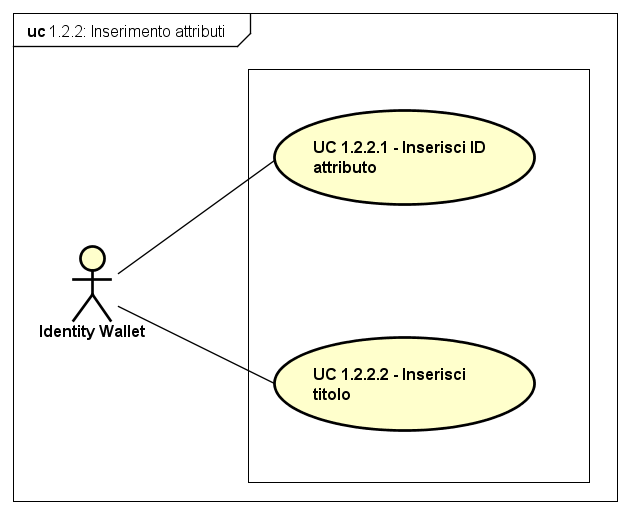
\includegraphics[scale=0.50]{immagini/usecase/UC122_InserimentoAttributi}
	\caption{Caso d'uso UC1.2.2: Insierimento attributi}
\end{figure}
\begin{itemize}
	\item \textbf{Descrizione} -L'Identity Wallet compila i campi dedicati agli attributi/certificazioni per creare l'identità digitale dell'utente;
	\item \textbf{Attori Principali} - Identity Wallet;
	\item \textbf{Attori Secondari} -
	\item \textbf{Pre-Condizioni} - L'Identity Wallet non possiede le informazioni inerenti agli attributi/certificazioni dell'utente che sta registrando nell'\gls{ITF};
	\item \textbf{Post-Condizioni} - L'Identity Wallet possiede tutte le informazioni inerenti agli attributi/certificazioni dell'utente che sta registrando nell'\gls{ITF};
	\item \textbf{Scenario Principale} -
	\begin{enumerate}
		\item Inserimento dell'ID che individua l'attributo (UC 1.2.2.1);
		\item Insierimento del titolo che descrive l'attributo (UC 1.2.2.2).
	\end{enumerate}
	\item \textbf{Estensioni} -
\end{itemize}
\subsection{Caso d'uso UC1.3: Aggiornamento attributi}
\begin{figure}[h]
	\centering
	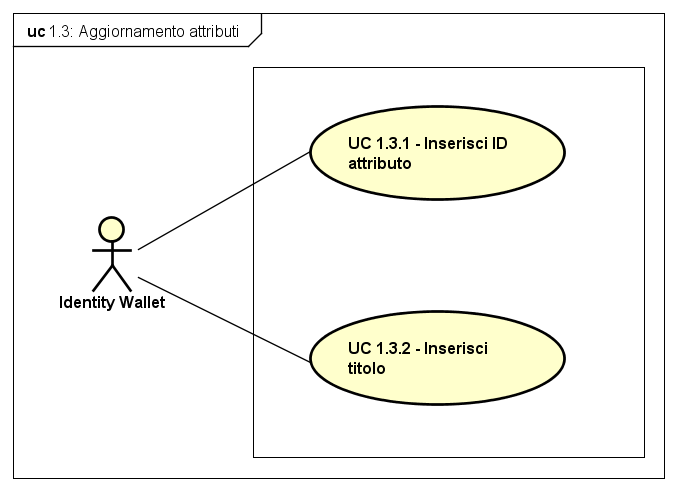
\includegraphics[scale=0.50]{immagini/usecase/UC13_AggiornamentoAttributi}
	\caption{Caso d'uso UC1.3: Aggiornamento attributi}
\end{figure}
\begin{itemize}
	\item \textbf{Descrizione} - L'Identity Wallet aggiorna gli attributi/certificazioni dell'utente, aggiungendone di nuove alla lista di quelle già presente nell'\gls{ITF};
	\item \textbf{Attori Principali} - Identity Wallet;
	\item \textbf{Attori Secondari} -
	\item \textbf{Pre-Condizioni} - L'Identity Wallet vuole aggiornare la lista di attributi/certificazioni associati all'utente;
	\item \textbf{Post-Condizioni} - L'Identity Wallet ha aggiornato la lista di attributi/certificazioni associati all'utente;
	\item \textbf{Scenario Principale} -
	\begin{enumerate}
		\item Inserimento dell'ID corrispondente all'attributo (UC 1.3.1);
		\item Inserimento del titolo descrittivo dell'attributo (UC 1.3.2).
	\end{enumerate}
	\item \textbf{Estensioni} -
\end{itemize}
\subsection{Caso d'uso UC1.4: Visualizza errore registrazione utente}
\begin{itemize}
	\item \textbf{Descrizione} - All'Identity Wallet viene segnalata, tramite un opportuno errore, l'impossibilità di creare e registrare una nuova identità digitale per l'utente. Questo avviene quando si tenta di registrare un'identità che è già presente nel sistema;
	\item \textbf{Attori Principali} - Identity Wallet;
	\item \textbf{Attori Secondari} -
	\item \textbf{Pre-Condizioni} - L'Identity Wallet vuole registrare una nuova identityà digitale per l'utente;
	\item \textbf{Post-Condizioni} - L'Identity Wallet non è riuscito a registrare la nuova identityà digitale nell'\gls{ITF};
	\item \textbf{Scenario Principale} -
	\begin{enumerate}
		\item All'Identity Wallet viene segnalata, tramite un errore, l'impossibilità di registrare il nuovo utente al sistema (UC 1.4);
	\end{enumerate}
	\item \textbf{Estensioni} -
\end{itemize}
\subsection{Caso d'uso UC1.5: Visualizza errore aggioranemento attributo}
\begin{itemize}
	\item \textbf{Descrizione} - All'Identity Wallet viene segnalata, tramite un opportuno errore, l'impossibilità di aggiornare la lista di attributi/certificazioni dell'utente. Questo avviene quando si tenta di aggiornare un attributo/certificazione che non è presente nell'\gls{ITF};
	\item \textbf{Attori Principali} - Identity Wallet;
	\item \textbf{Attori Secondari} -
	\item \textbf{Pre-Condizioni} - L'Identity Wallet vuole aggiornare la lista degli attributi e certificazioni associati all'utente;
	\item \textbf{Post-Condizioni} - La lista non è stata aggiornata;
	\item \textbf{Scenario Principale} -
	\begin{enumerate}
		\item All'Identity Wallet viene segnalata, tramite un errore, l'impossibilità di agiornare gli attributi (UC 1.5);
	\end{enumerate}
	\item \textbf{Estensioni} -
\end{itemize}
\subsection{Caso d'uso UC2: Certificazione}
\begin{figure}[h]
	\centering
	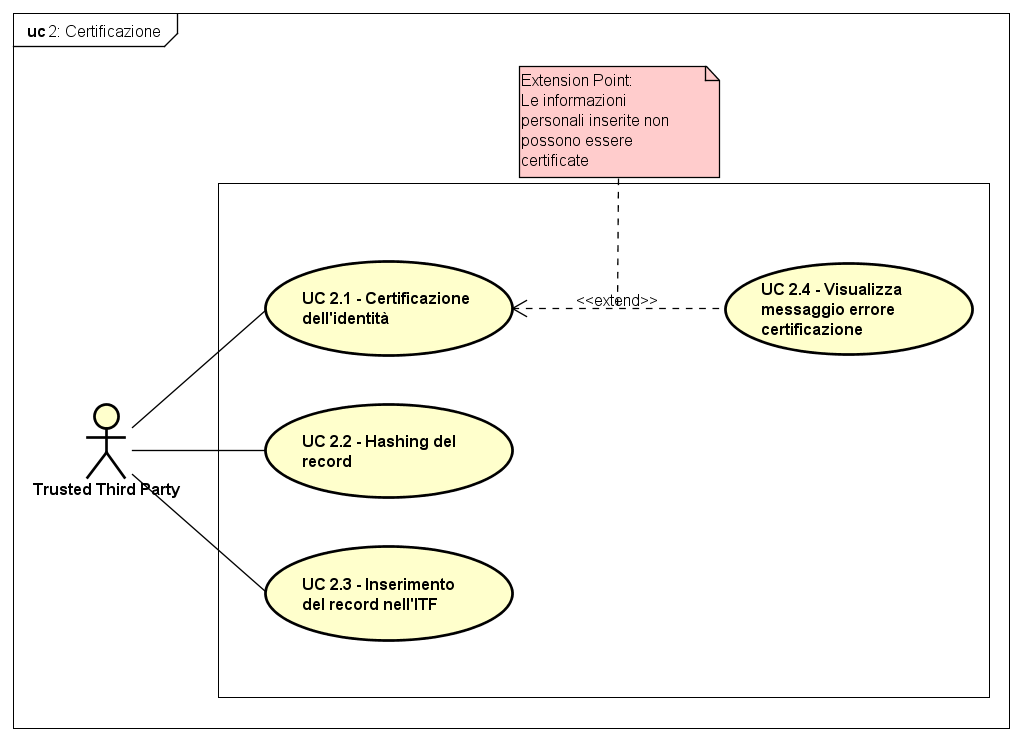
\includegraphics[scale=0.50]{immagini/usecase/UC2_Certificazione}
	\caption{Caso d'uso UC2: Certificazione}
\end{figure}
\begin{itemize}
	\item \textbf{Descrizione} - L'attore vuole certificare tutte le informazioni riguardanti l'identità digitale dell'utente e, una volta certificate, inserirle nell'\gls{ITF}.\\
	La certificazione avviene grazie alla firma, delle informazioni personali e degli attributi, tramite la chiave privata dell'attore. Una volta firmate, le informazioni vengono inserite in un record, fatto l'\textit{hash} del record e quindi inserito nell'\gls{ITF};	
	\item \textbf{Attori Principali} - Trusted Third Party;
	\item \textbf{Attori Secondari} -
	\item \textbf{Pre-Condizioni} - L'attore vuole certificare l'identità e gli attributi di un particolare utente;
	\item \textbf{Post-Condizioni} - La Trusted Third Party ha certificato correttamente l'identità e gli attributi dell'utente e ha inserito il record nell'\gls{ITF};
	\item \textbf{Scenario Principale} -
	\begin{enumerate}
		\item L'attore certifica le informazioni dell'utente (UC 2.1);
		\item L'attore esegue l'\textit{hash} del record contenente tutte le informazioni appena certificate (UC 2.2);
		\item L'attore, una volta fatto l'\textit{hash} del record, lo inserisce nell'\gls{ITF} (UC 2.3).
	\end{enumerate}
	\item \textbf{Estensioni} -
	\begin{enumerate}
		\item Visualizza messaggio d'errore nella certificazione delle informazioni personali (UC 2.4).
	\end{enumerate}
\end{itemize}
\subsection{Caso d'uso UC2.1: Certificazione dell'identità}
\begin{figure}[h]
	\centering
	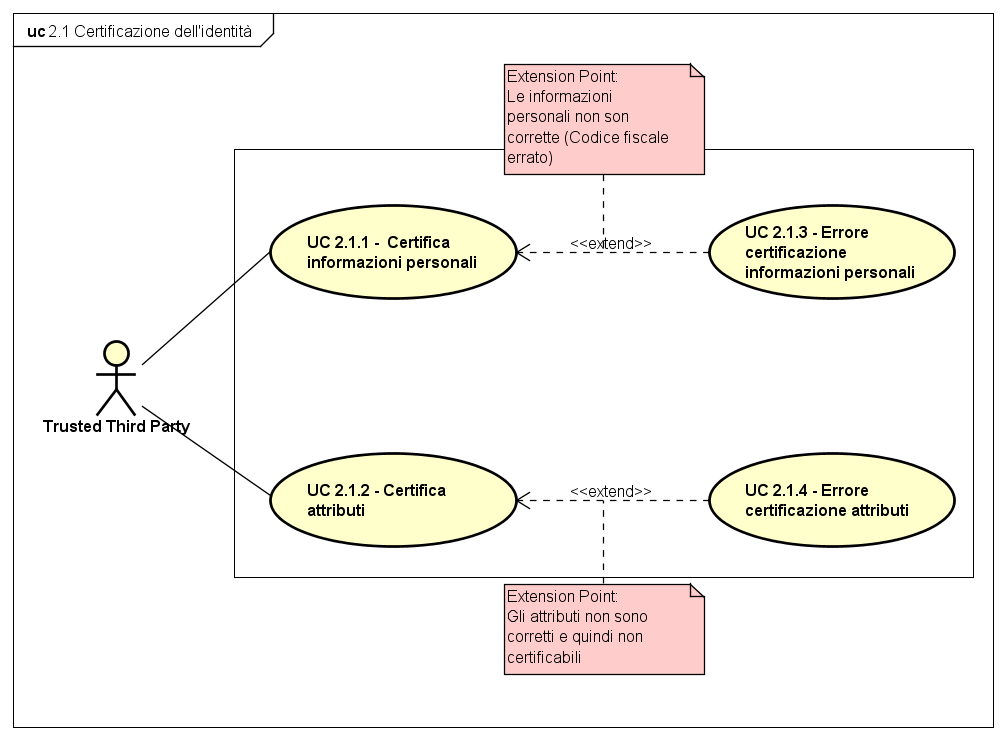
\includegraphics[scale=0.50]{immagini/usecase/UC21_CertificazioneIdentita}
	\caption{Caso d'uso UC2.1: Certificazione dell'identità}
\end{figure}
\begin{itemize}
	\item \textbf{Descrizione} - La Trusted Third Party, prima di inserire il record nell'ITF, deve certificare tutte le informazioni personali associate all'utente (dati e attributi/certificazioni).\\
	Questo viene fatto grazie alla firma, dei dati e degli attributi, tramite chiave privata della Trusted Third Party;
	\item \textbf{Attori Principali} - Trusted Third Party;
	\item \textbf{Attori Secondari} -
	\item \textbf{Pre-Condizioni} - L'attore vuole certificare tutte le informazioni personali dell'utente;
	\item \textbf{Post-Condizioni} - L'attore ha certificato tutte le informazioni personali dell'utente;
	\item \textbf{Scenario Principale} -
	\begin{enumerate}
		\item Certificazione delle informazioni personali tramite chiave privata (UC 2.1.1);
		\item Certificazione degli attributi/certificazioni tramite chiave privata (UC 2.1.2).
	\end{enumerate}
	\item \textbf{Estensioni} -
	\begin{enumerate}
		\item Visualizza errore nella certificazione delle informazioni personali (UC 2.1.3);
		\item Visualizza errore nella certificazione degli attributi (UC 2.1.4).
	\end{enumerate}
\end{itemize}
\subsection{Caso d'uso UC 2.4: Visualizza errore certificazione dell'identità}
\begin{itemize}
	\item \textbf{Descrizione} - Alla Trusted Third Party viene segnalata l'impossibilità di certificare uno o più informazioni personali dell'utente (dati personali, attributo o certificazioni).\\
	Questo avviene quando, la Trusted Third Party, non riesce a trovare corrispondenza tra gli attributi e i dati indicati con l'identità dell'utente;
	\item \textbf{Attori Principali} - Trusted Third Party;
	\item \textbf{Attori Secondari} - L'attore vuole certificare tutte le informazioni personali dell'utente (dati personali e attributi);
	\item \textbf{Pre-Condizioni} -
	\item \textbf{Post-Condizioni} - L'attore non è riuscito a certificare gli attributi e/o i dati personali dell'utente;
	\item \textbf{Scenario Principale} -
	\begin{enumerate}
		\item L'attore viene segnalato dell'impossibilità di certificare le informazioni personlai dell'utente, tramite un apposito errore (UC 2.4).
	\end{enumerate}
	\item \textbf{Estensioni} -
\end{itemize}
\subsection{Caso d'uso UC 2.1.3: Visualizza errore certificazione informazioni personali}
\begin{itemize}
	\item \textbf{Descrizione} - Alla Trusted Third Party viene segnalata l'impossibilità di certificare le informazoni personali dell'utente;
	\item \textbf{Attori Principali} - Trusted Third Party
	\item \textbf{Attori Secondari} -
	\item \textbf{Pre-Condizioni} - L'attore vuole certificare le informazioni personali dell'utente;
	\item \textbf{Post-Condizioni} - L'attore non è riuscito a certificare le informazioni personali dell'utente;
	\item \textbf{Scenario Principale} -
	\begin{enumerate}
		\item L'attore viene senglatao dell'impossibilità di certificare le informazioni personali, tramite un apposito errore (UC 2.1.3).
	\end{enumerate}
	\item \textbf{Estensioni} -
\end{itemize}
\subsection{Caso d'uso UC 2.1.4: Visualizza errore certificazione attributi}
\begin{itemize}
	\item \textbf{Descrizione} - Alla Trusted Third Party viene segnalata l'impossibilità di certificare gli attributi dell'utente;
	\item \textbf{Attori Principali} - Trusted Third Party;
	\item \textbf{Attori Secondari} -
	\item \textbf{Pre-Condizioni} - L'attore vuole certificare gli attributi dell'utente;
	\item \textbf{Post-Condizioni} - L'attore non è riuscito a certificare gli attributi dell'utente;
	\item \textbf{Scenario Principale} - 
	\begin{enumerate}
		\item L'attore viene segnalato dell'impossibilità di certificare gli attributi, trmaite un apposito errore (UC 2.1.4).
	\end{enumerate}
	\item \textbf{Estensioni} -
\end{itemize}
\subsection{Caso d'uso UC3: Verifica dell'identità}
\begin{figure}[h]
	\centering
	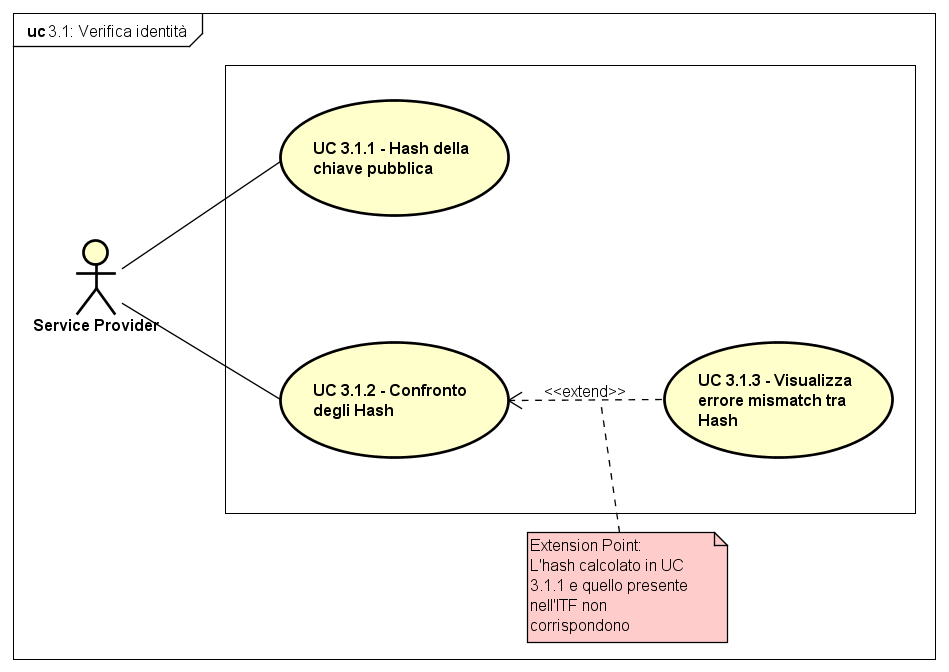
\includegraphics[scale=0.50]{immagini/usecase/UC31_VerificaIdentita}
	\caption{Caso d'uso UC3: Verifica}
\end{figure}
\begin{itemize}
	\item \textbf{Descrizione} - Il Service Provider, prima di poter erogare i suoi servizi, deve accertarsi che l'utente sia in possesso delle credenziali e degli attributi necessari. Questo avviene tramite la verifica dell'identità e la verifica degli attributi presenti nell'\gls{ITF};
	\item \textbf{Attori Principali} -Service Provider;
	\item \textbf{Attori Secondari} -
	\item \textbf{Pre-Condizioni} - Il Service Provider non ha verificato l'identità e gli attributi dell'utente;
	\item \textbf{Post-Condizioni} - Il Service Provider ha verificato l'identità dell'utente e può erogare i suoi servizi;
	\item \textbf{Scenario Principale} -
	\begin{enumerate}
		\item Verifica dell'identità dell'utente (UC 3.1);
		\item Verfica degli attributi dell'utente (UC 3.2).
	\end{enumerate}
	\item \textbf{Estensioni} -
	\begin{enumerate}
		\item Visualizza errore nella verifica dell'identità (UC 3.3);
		\item Visualizza errore nella verifica degli attributi (UC 3.4).
	\end{enumerate}
\end{itemize}
\subsection{Caso d'uso UC3.1: Verifica identità}
\begin{figure}[h]
	\centering
	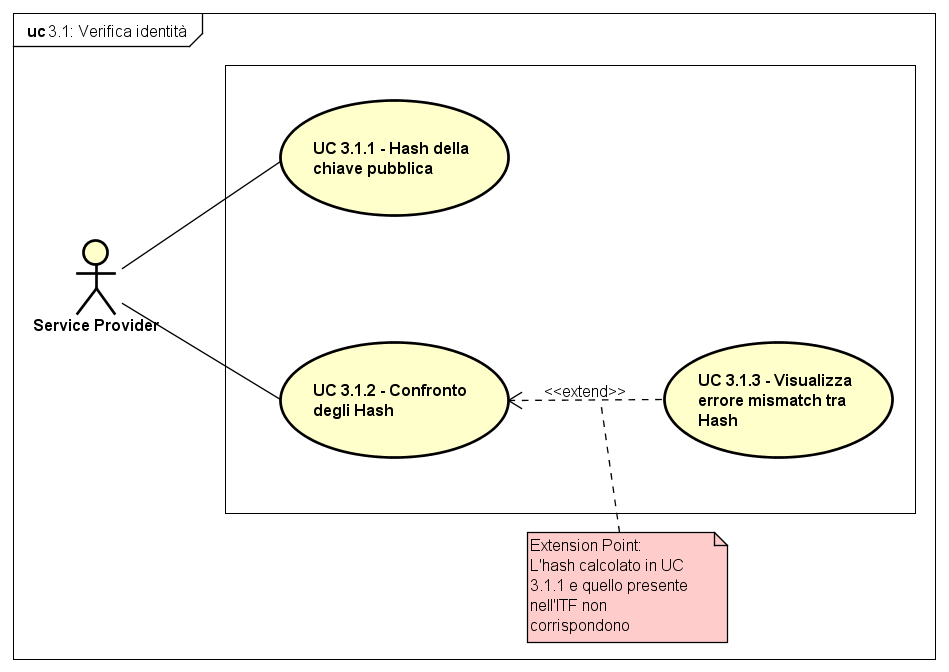
\includegraphics[scale=0.50]{immagini/usecase/UC31_VerificaIdentita}
	\caption{Caso d'uso UC3.1: Verifica dell'identità}
\end{figure}
\begin{itemize}
	\item \textbf{Descrizione} -  Il Service Provider, prima di permettere all'utente di usufruire dei suoi servizi, deve accertarsi che l'identità dell'utente sia corretta rispetto a quella presente nell'\gls{ITF};
	\item \textbf{Attori Principali} - Service Provider;
	\item \textbf{Attori Secondari} -
	\item \textbf{Pre-Condizioni} - L'attore non sa se può erogare i servizi all'utente;
	\item \textbf{Post-Condizioni} - Il Service Provider ha verificato l'identità dell'utente e può erogare i suoi servizi;
	\item \textbf{Scenario Principale} -
	\begin{enumerate}
		\item \textit{Hash} della chiave pubblica passata dall'Idenitity Wallet (UC 3.1.1);
		\item Confronto del \textit{hash} calcolato in UC 3.1.1 con quello presente nell'\gls{ITF} (UC 3.1.2).
	\end{enumerate}
	\item \textbf{Estensioni} -
	\begin{enumerate}
		\item Visualizza errore mismatch degli hash (UC 3.1.3).
	\end{enumerate}
\end{itemize}
\subsection{Caso d'uso UC3.3: Visualizza errore verifica dell'identità}
\subsection{Caso d'uso UC3.1.3: Visualizza errore mismatch degli hash}
\subsection{Caso d'uso UC3.4: Visualizza errore verifica degli attributi}